\section{StarLight}
\label{sec:ComposestarStarLight}

In 2006 development began on a lightweight branch of \Compose*[.NET], called StarLight. The aim of this new branch is to provide a more robust and efficient variant of \Compose*. Certain more advanced features, such as multiple inheritance, have been excluded from this new branch, while new features have been implemented to meet industry demands. This section describes the differences in the architecture between \Compose* and StarLight and certain new features of StarLight.

\subsection{StarLight Architecture}
This section describes differences between the StarLight Architecture and the \Compose* architecture, as shown in \autoref{fig:ComposestarArchitecture}.
\begin{description}[style=nextline]
\item[Integrated Development Environment]
StarLight has its own Visual Studio integration. This integration provides the following functionality:
\begin{itemize}[noitemsep]
\item A project service to open and use StarLight projects in Visual Studio;
\item Syntax highlighting and IntelliSense for concern files;
\item MSBuild is used to analyze and weave the concerns. 
\end{itemize}
\item[Compile Time]
StarLight uses the same compile time as \Compose*. An inlining engine is added to the compile time. This inlining engine translates the filter set to a platform independent abstract instruction model for each individual message. This abstract instruction model represents a procedural structure. It can be easily translated to program code for a specific procedural platform.
\item[Adaptation]
StarLight has its own adaptation layer. It contains an analyzer that creates the language model. It also contains a weaver that translates the abstract instruction models for each message to IL code and weaves this code in the appropriate places of the target assemblies.
\item[Runtime]
The StarLight version does not have a runtime, because a complete filter set translation is woven in the target program.
\end{description}

\subsection{Explicit Modeling of the Returning Flow}
\begin{figure}[htbp]
  \centering
  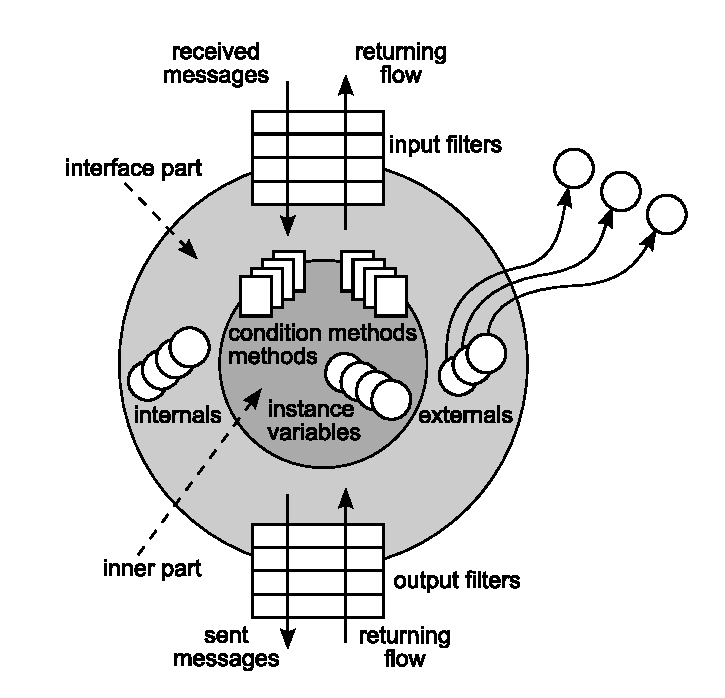
\includegraphics[style=thirdheight]{cfmodelreturningflow}
  \caption{Explicit modeling of the returning flow}
  \label{fig:cfmodelreturningflow}
\end{figure}

Originally, composition filters only modeled the calling flow: sending the message from the sender to the target. There is, however, also a returning flow: the action of returning the control to the sender after the target has ended the execution of the message. This returning flow possibly contains a return value, but this is not necessary. In the new StarLight implementation we also want to model this returning flow explicitly. This makes it possible to execute filter actions after the message has been dispatched.

\autoref{fig:cfmodelreturningflow} shows the returning flow in the composition filters model. Both input filters as output filters have a returning flow.

\paragraph{When is the Flow Returned?}
Explicit modeling of the returning flow raises questions like when is the flow returned and is there always a returning flow. From the composition filters perspective, it is the filter action that decides whether to return the flow or to continue to the next filter. There are actually three possibilities, as shown in \autoref{fig:filteractionflowbehavior}.

\begin{figure}[htbp]
  \centering
  \subfloat[Continue]{
    \includegraphics[scale=0.70]{ContinueAction.pdf} 
  }\qquad
  \subfloat[Return]{
    \includegraphics[scale=0.70]{ReturnAction.pdf} 
  }\qquad
  \subfloat[Exit]{
    \includegraphics[scale=0.70]{ExitAction.pdf} 
  }
  \caption[Filter actions can either continue, return or exit]{Filter actions can either continue, return or exit.}
  \label{fig:filteractionflowbehavior}
\end{figure}

\begin{description}[style=nextline, noitemsep]
\item[Continue]
The flow continues to the next filter. Examples of filter actions that continue the flow are the \lstinline|Substitution| action and the \lstinline|Advice| action.
\item[Return]
A filter action can return the flow. In this case, the calling flow turns into a returning flow. An example of a filter action that returns the flow is the \lstinline|Dispatch| action.
\item[Exit]
The third option available for filter actions is to exit the filter set. This equals an exception or abnormal return. An example of a filter action that exits the filter set is the \lstinline|Error| action.
\end{description}

\paragraph{4-Action Filter Types}
Because StarLight models the returning flow explicitly, it is possible to execute actions on the returning flow. The actions that are executed, are specified by the filter type. Therefore, instead of 2-action filter types, StarLight has 4-action filter types.
\begin{table}[htbp]
\begin{center}
\begin{tabular}{lrr}
 & Calling Flow& Returning Flow \\\hline
Accept & accept-call action & accept-return action\\
Reject & reject-call action & reject-return action\\
\end{tabular}
\end{center}
\caption{The four filter actions of a filter type.}
\label{tab:fourfilteractions}
\end{table}

\paragraph{Evaluation of Filters on the Returning Flow?}
The filters are not evaluated on the returning flow. They are only evaluated on the calling flow. The filter action that is executed by a filter on the returning flow depends on whether the filter accepted or rejected on the calling flow.

The actions on the returning flow are executed in reverse order of the filter set.

\subsection{Defining New Filter Types and Filter Actions}
StarLight provides a new way to define new filter types and new filter actions. Actually, there are no primitive filter types and filter actions anymore, as there are in \Compose*. There are, however, certain common filter types and filter actions provided by the StarLight API. But they are defined in the same way as any other new filter type or filter action.


\begin{lstlisting}[language={[Sharp]C},style=listing,caption={Defining the \expandafter{\lstinline|LoggingIn|} filter actions},label={lst:loggingactionsexample}]
[FilterActionAttribute("LoggingInAction", FilterActionAttribute.FilterFlowBehavior.Continue, FilterActionAttribute.MessageSubstitutionBehavior.Original)]
public class LoggingInAction : FilterAction
{
	public override void Execute(JoinPointContext context)
	{
		//Logging-in implementation
	}
} 
\end{lstlisting} 

New filter actions can be defined by extending the \lstinline|FilterAction| class. \autoref{lst:loggingactionsexample} shows an example of a new filter action. By overriding the \lstinline|Execute| method, the action can be implemented. When the action is executed at runtime, a call is done to its \lstinline|Execute| method. A mandatory custom attribute on the filter action specifies the following information:
\begin{itemize}[noitemsep]
\item The name of the filter action;
\item The flow behavior of the filter action: continue, return or exit;
\item The substitution behavior of the filter action. This specifies whether the message continues substituted or not after the filter action. An example of a filter action that leaves the message substituted is the \lstinline|Substitution| action.
\end{itemize}

\begin{lstlisting}[language={[Sharp]C},style=listing,caption={Defining the \expandafter{\lstinline|Logging|} filter type},label={lst:loggingfiltertypeexample}]
[FilterTypeAttribute("Logging", "LoggingInAction", FilterAction.ContinueAction, "LoggingOutAction",FilterAction.ContinueAction)]
class LoggingFilterType : FilterType
{
	//No implementation
}
\end{lstlisting} 
A new filter type can be defined by extending the \lstinline|FilterType| class. \autoref{lst:loggingfiltertypeexample} shows an example of a new filter type. This class has no implementation methods, as it is not used at runtime. It is only used to specify a new filter type at compile time. A mandatory custom attribute specifies the following information:
\begin{itemize}[noitemsep]
\item The name of the filter type. This name can be used in filter specifications;
\item The filter actions, in the order accept-call, reject-call, accept-return and reject-return.
\end{itemize}
The example shows the definition of a \lstinline|Logging| filter type that logs both on call as on return, when the filter accepts.


\subsubsection{Built-in Filter Actions}
The StarLight API provides several filter actions:

\begin{description}[style=sameline,leftmargin=28mm]
 \item[Continue] This filter action continues the execution of the filter set to the next filter. It does not have any other behavior
  \item[Dispatch] This action dispatches the message to the specified target.
  \item[Advice] This action executes a specific advice method, specified by the substitution part. This is a lightweight replacement of the \lstinline|Meta| action. It cannot change the message or change the flow behavior of the message. It also does not have the multithreading functionality of the \lstinline|Meta| action. After an \lstinline|Advice| action, the flow continues to the next filter with an unchanged message.
  \item[Error] This action raises an exception and causes the flow to exit the filter set.
  \item[Substitution] This action substitutes the message with the message specified by the substitution part. The execution of the filter set continues to the next filter.
\end{description}

\subsubsection{Built-in Filter Types}
The StarLight API provides several filter types:
% These are shown in \autoref{tab:filtertypesstarlight}.
\begin{description}[style=sameline,leftmargin=28mm]
\item[Dispatch]
\begin{tabular}{lrr}
 & Calling Flow& Returning Flow \\\hline
Accept & Dispatch action & Continue action\\
Reject & Continue action & Continue action\\
\end{tabular}

\item[Before]
\begin{tabular}{lrr}
 & Calling Flow& Returning Flow \\\hline
Accept & Advice action & Continue action\\
Reject & Continue action & Continue action\\
\end{tabular}

\item[After]
\begin{tabular}{lrr}
 & Calling Flow& Returning Flow \\\hline
Accept & Continue action & Advice action\\
Reject & Continue action & Continue action\\
\end{tabular}

\item[Error]
\begin{tabular}{lrr}
 & Calling Flow& Returning Flow \\\hline
Accept & Error action & Continue action\\
Reject & Continue action & Continue action\\
\end{tabular}

\item[Substitution]
\begin{tabular}{lrr}
 & Calling Flow& Returning Flow \\\hline
Accept & Subst. action & Continue action\\
Reject & Continue action & Continue action\\
\end{tabular}
\end{description}


\subsection{Conditional Superimposition}
Another new feature in the StarLight version of \Compose* is conditional superimposition. Conditional superimposition makes it possible to superimpose a filter module conditionally. At runtime the condition is evaluated to decide whether the filter module should be executed. This makes it possible to turn crosscutting behavior on and off at runtime. It is even possible to turn the filter module off for specific classes, because the condition can get the classname as parameter.

\begin{lstlisting}[language=Composestar,style=listing, caption={Conditional superimposition example},label={lst:condsuperimpexample}]
concern LoggingConcern
{
	filtermodule LoggingFM
	{
		inputfilters
			logging  : Logging = { True => [*.*] }
	}
	
	superimposition
	{
		conditions
		    loggingEnabled : Logging.LoggingEnabled;
		selectors
			loggingClasses = { ... };
		filtermodules
			loggingEnabled => loggingClasses <- LoggingFM;
	}
}
\end{lstlisting}
\autoref{lst:condsuperimpexample} shows an example of conditional superimposition. In this example, the \lstinline|LoggingFM| filter module is superimposed conditionally. Before the filter module is executed at runtime, the condition \lstinline|loggingEnabled| is checked.